\documentclass[11pt,a4paper]{article}

\usepackage[utf8]{inputenc}
\usepackage[T1]{fontenc}
\usepackage{lmodern}
\usepackage[margin=2.2cm]{geometry}
\usepackage{xcolor}
\usepackage{booktabs}
\usepackage{parskip}
\usepackage{fancyhdr}
\usepackage{tikz}
\usetikzlibrary{arrows.meta, positioning, shapes.geometric}
\usepackage{hyperref}

\definecolor{PrimaryBlue}{HTML}{1E3A5F}
\definecolor{AccentTeal}{HTML}{0F766E}
\definecolor{SoftBg}{HTML}{F1F5F9}
\definecolor{WarmAmber}{HTML}{B45309}
\definecolor{BorderGray}{HTML}{CBD5E1}

\hypersetup{
    colorlinks=true,
    linkcolor=PrimaryBlue,
    urlcolor=AccentTeal,
    pdftitle={Whispernet - Architecture de Securite (Authenticite et Privacite)}
}

\pagestyle{fancy}
\fancyhf{}
\lhead{\small\color{PrimaryBlue}\textbf{Whispernet} — Sécurité : Authenticité et Privacité}
\rhead{\small\color{AccentTeal}Architecture Cryptographique}
\cfoot{\small\thepage}

\title{\textbf{\color{PrimaryBlue}Whispernet — Choix de Sécurité}\\[0.3em]\large Authenticité, Intégrité et Privacité des Données et des Groupes}
\author{Équipe Whispernet}
\date{\today}

\begin{document}
\maketitle

\section{Vue d'ensemble des choix de sécurité}

Whispernet repose sur une architecture décentralisée sans serveur central. La sécurité est découpée en deux axes complémentaires :
\begin{enumerate}
    \item \textbf{Authenticité et intégrité} : prouver qui a créé un compte, un groupe, une règle de modération ou un message, tout en empêchant toute falsification en transit.
    \item \textbf{Privacité et confidentialité} : protéger les clés privées et fichiers locaux au repos, chiffrer les liens pair-à-pair et isoler les groupes entre eux.
\end{enumerate}

\begin{center}
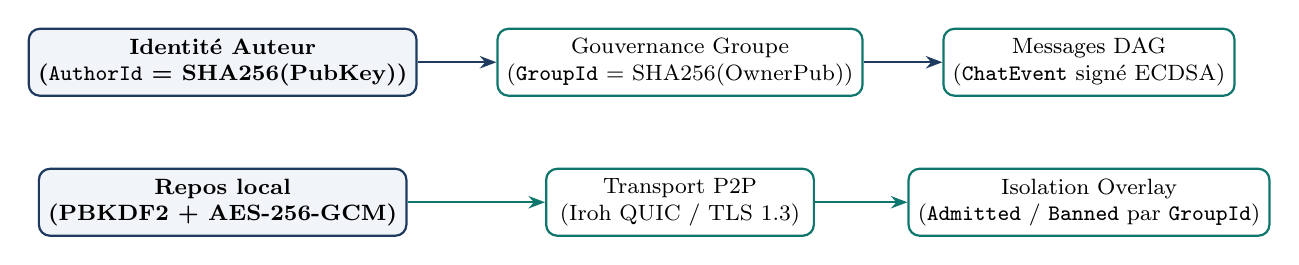
\begin{tikzpicture}[
    node distance=0.6cm and 0.9cm,
    box/.style={rectangle, draw=PrimaryBlue, thick, fill=SoftBg, rounded corners=4pt, minimum width=3.4cm, minimum height=0.85cm, align=center, font=\footnotesize\bfseries},
    sec/.style={rectangle, draw=AccentTeal, thick, fill=white, rounded corners=4pt, minimum width=3.4cm, minimum height=0.85cm, align=center, font=\footnotesize},
    arr/.style={-{Stealth[length=2.1mm]}, thick, PrimaryBlue}
]
    \node[box] (auth) {Identité Auteur\\(\texttt{AuthorId} = SHA256(PubKey))};
    \node[sec, right=1.0cm of auth] (grp) {Gouvernance Groupe\\(\texttt{GroupId} = SHA256(OwnerPub))};
    \node[sec, right=1.0cm of grp] (dag) {Messages DAG\\(\texttt{ChatEvent} signé ECDSA)};

    \node[box, below=0.9cm of auth] (vault) {Repos local\\(PBKDF2 + AES-256-GCM)};
    \node[sec, below=0.9cm of grp] (quic) {Transport P2P\\(Iroh QUIC / TLS 1.3)};
    \node[sec, below=0.9cm of dag] (iso) {Isolation Overlay\\(\texttt{Admitted} / \texttt{Banned} par \texttt{GroupId})};

    \draw[arr] (auth) -- (grp);
    \draw[arr] (grp) -- (dag);
    \draw[arr, AccentTeal] (vault) -- (quic);
    \draw[arr, AccentTeal] (quic) -- (iso);
\end{tikzpicture}
\end{center}

\section{Authenticité et Intégrité}

\subsection{Identité d'auteur séparée de l'identité réseau}
L'identité réseau d'un appareil (\texttt{NodeId} Ed25519 géré par Iroh) est découplée de l'identité applicative de l'utilisateur (\texttt{AuthorId}).
\begin{itemize}
    \item \textbf{Algorithme} : \textbf{ECDSA sur la courbe NIST P-256} (\texttt{System.Security.Cryptography.ECDsa}), exportée au format standard SPKI DER (clé publique) et PKCS\#8 DER (clé privée).
    \item \textbf{Méthodes concernées} :
    \begin{itemize}
        \item \texttt{AccountService.CreateAccountAsync} : génère la paire ECDSA P-256.
        \item \texttt{AccountCrypto.ComputeAuthorId} : calcule \texttt{AuthorId = SHA256(PublicKeySpki)} (64 caractères hexadécimaux).
        \item \texttt{AccountService.SignData} / \texttt{AccountService.VerifySignature} : signe et vérifie toute donnée applicative avec \texttt{HashAlgorithmName.SHA256}.
    \end{itemize}
\end{itemize}

\subsection{Authenticité des groupes et modération (CRDT LWW)}
À la création d'un groupe, une \textbf{paire de clés ECDSA P-256 dédiée au groupe} (distincte de la clé personnelle \texttt{AuthorId} de l'utilisateur) est générée : seul l'administrateur en possède la clé privée, ce qui lui permet de créer un nombre illimité de groupes indépendants. Le groupe est ancré à cette clé dédiée : \texttt{GroupId = SHA256(GroupPublicKeySpki)}.
\begin{itemize}
    \item \textbf{Règles du groupe (\texttt{GroupManifest})} : seul l'administrateur détient la clé privée du groupe correspondant à \texttt{GroupId} et peut signer les mises à jour (titre, modérateurs, mot de passe d'admission, durée éphémère ou fermeture définitive \texttt{IsTerminated}).
    \item \textbf{Modération et liste d'admis (\texttt{ModerationAction})} : seuls l'administrateur (via sa clé de groupe ou son \texttt{AuthorId} inscrit dans les modérateurs) ou les modérateurs listés dans la version courante du manifeste peuvent signer des changements de statut (\texttt{Admitted}, \texttt{Silenced}, \texttt{Banned}).
    \item \textbf{Protection anti-usurpation et anti-modérateur révoqué} : chaque action est liée à \texttt{ManifestVersion} et validée sur sa représentation binaire canonique.
    \item \textbf{Méthodes concernées} :
    \begin{itemize}
        \item \texttt{GroupId.FromOwnerPublicKeySpki} : dérive et vérifie l'ancrage du groupe.
        \item \texttt{GroupManifest.BuildSignableBytes} et \texttt{ModerationAction.BuildSignableBytes} : sérialisation binaire préfixée en longueur (sans ambiguïté).
        \item \texttt{GroupGovernanceEngine.TryApplyManifest} : vérifie \texttt{SHA256(OwnerPubKey) == GroupId}, la monotonie de \texttt{Version}, l'irréversibilité de \texttt{IsTerminated} et la signature du créateur.
        \item \texttt{GroupGovernanceEngine.TryApplyModerationAction} : vérifie que le signataire est le créateur ou un modérateur actif, valide la signature ECDSA, puis applique la convergence déterministe \emph{Last-Write-Wins} \texttt{(LamportClock, IssuedAtUtc, SignerAuthorId)}.
        \item \texttt{GroupGovernanceService.CreateGroupAsync} et \texttt{UpdateGroupManifestAsync} : génère la paire ECDSA P-256 dédiée au groupe, efface les tampons privés via \texttt{ZeroMemory} et signe les mises à jour.
        \item \texttt{GroupGovernanceService.TryProcessJoinApprovalRequest} et \texttt{VerifyJoinPassword} : valide la signature de \texttt{JoinApprovalRequest}, vérifie le mot de passe d'admission en temps constant (\texttt{CryptographicOperations.FixedTimeEquals} sur PBKDF2-HMAC-SHA256 à 600\,000 itérations) et rejette les comptes \texttt{Banned}.
        \item \texttt{GroupMeshService.ApplySyncPayload} : valide cryptographiquement chaque manifeste et action lors de la synchronisation anti-entropie.
    \end{itemize}
\end{itemize}

\subsection{Authenticité et causalité des messages (\texttt{ChatEvent} DAG)}
Chaque message est un nœud immuable du DAG causal du salon :
\begin{itemize}
    \item \textbf{Hash d'intégrité} : \texttt{event\_id = SHA-256(parents || payload)} lie de façon cryptographique le contenu à ses antécédents causaux (max 15 parents).
    \item \textbf{Méthodes concernées} :
    \begin{itemize}
        \item \texttt{ChatEvent.ComputeEventId} et \texttt{ChatEvent.BuildSignableBytes}.
        \item \texttt{ChatEventService.CreateSignedEvent} : calcule \texttt{event\_id} et signe l'événement complet via \texttt{AccountSession}.
        \item \texttt{CausalDagEngine.TryIngestEvent} : vérifie la limite de 15 parents, la cohérence de \texttt{logical\_clock}, l'intégrité de \texttt{event\_id} et la signature ECDSA avant d'insérer et de trier le message.
    \end{itemize}
\end{itemize}

\section{Privacité et Confidentialité}

\subsection{Protection des clés et du coffre local au repos}
Lorsqu'un utilisateur définit un mot de passe optionnel à la création du compte :
\begin{itemize}
    \item \textbf{Dérivation de clé} : \textbf{PBKDF2-HMAC-SHA256} avec \textbf{600\,000 itérations} et un sel aléatoire de 16 octets produit la clé maître (\texttt{KEK} 256 bits). Aucun mot de passe ni condensat de mot de passe n'est enregistré sur disque.
    \item \textbf{Enveloppe KEK / DEK et chiffrement authentifié} : \textbf{AES-256-GCM} (nonce aléatoire 12 octets, tag d'authentification 16 octets, \emph{Associated Data} AAD liant l'\texttt{AuthorId} et le chemin relatif du fichier).
    \item \textbf{Méthodes concernées} :
    \begin{itemize}
        \item \texttt{AccountCrypto.DeriveKeyFromPassword} : dérivation PBKDF2 avec effacement immédiat des octets du mot de passe.
        \item \texttt{AccountCrypto.EncryptAesGcm} / \texttt{AccountCrypto.DecryptAesGcm} : chiffrement authentifié avec détection immédiate de toute altération ou mauvais mot de passe (\texttt{CryptographicException}).
        \item \texttt{AccountService.WriteVaultFileAsync} / \texttt{ReadVaultFileAsync} : chiffre les fichiers dans \texttt{vault/} et bloque toute traversée de chemin (\texttt{ResolveVaultFilePath}).
        \item \texttt{GroupGovernanceService.SaveGroupToVaultAsync} / \texttt{LoadGroupFromVaultAsync} : stocke la clé privée dédiée d'un groupe dans \texttt{vault/groups/<groupId>.json} chiffré par le coffre du compte.
        \item \texttt{AccountSession.Dispose} : efface la \texttt{DEK} en RAM via \texttt{CryptographicOperations.ZeroMemory}.
        \item \texttt{AccountCrypto.ApplyRestrictivePermissions} : applique \texttt{0700} sur les dossiers et \texttt{0600} sur les fichiers sous Linux/macOS.
    \end{itemize}
\end{itemize}

\subsection{Privacité réseau et isolation des groupes}
\begin{itemize}
    \item \textbf{Chiffrement de transport} : toutes les connexions pair-à-pair Iroh utilisent \textbf{QUIC / TLS 1.3} (\texttt{IrohEndpointAdapter}), rendant le trafic illisible sur le réseau.
    \item \textbf{Contrôle d'accès par groupe} :
    \begin{itemize}
        \item \texttt{GroupGovernanceEngine.CanAuthorReceive} : n'autorise l'accès au flux d'un salon qu'aux \texttt{AuthorId} ayant le statut \texttt{Admitted} ou \texttt{Silenced} ; les comptes \texttt{Banned} ou \texttt{Unknown} sont rejetés.
        \item \texttt{GroupGovernanceEngine.CanAuthorPost} et \texttt{GroupMeshService.CanAcceptGroupPost} : filtrent dès le premier saut les messages d'auteurs \texttt{Silenced}, \texttt{Banned} ou \texttt{Unknown}, ainsi que les messages expirés (\texttt{EphemeralMessageTtl}).
        \item \texttt{GroupGovernanceState.GetRoomMemberEndpoints} et \texttt{GroupMeshService.GetReconnectTargets} : ne partagent les \texttt{EndpointId} des participants qu'entre membres admis du même salon.
        \item \texttt{GroupMeshService.ShouldClosePhysicalConnection} : isole les groupes par \texttt{GroupId} et gère le comptage de références QUIC à l'intersection de plusieurs groupes sans exposer un groupe à un autre.
    \end{itemize}
\end{itemize}

\section{Synthèse des primitives et méthodes}

\begin{center}
\footnotesize
\begin{tabular}{@{}llp{5.8cm}@{}}
\toprule
\textbf{Objectif} & \textbf{Primitive} & \textbf{Méthodes clés} \\
\midrule
Authenticité auteur & ECDSA P-256 + SHA-256 & \texttt{CreateAccountAsync}, \texttt{ComputeAuthorId}, \texttt{SignData} \\
Authenticité groupe & ECDSA P-256 + CRDT LWW & \texttt{TryApplyManifest}, \texttt{TryApplyModerationAction} \\
Intégrité messages & SHA-256 + ECDSA P-256 & \texttt{ComputeEventId}, \texttt{TryIngestEvent} \\
Privacité au repos & PBKDF2 (600k) + AES-256-GCM & \texttt{DeriveKeyFromPassword}, \texttt{EncryptAesGcm}, \texttt{ZeroMemory} \\
Privacité réseau & QUIC TLS 1.3 + Liste d'admis & \texttt{CanAuthorReceive}, \texttt{CanAuthorPost}, \texttt{GroupMeshService} \\
\bottomrule
\end{tabular}
\end{center}

\end{document}